\documentclass[a4paper,11pt]{article}
%\VignetteIndexEntry{StickPTW}

\usepackage{natbib}
\usepackage{geometry}
\usepackage{layout}
\usepackage{url}
\usepackage{Sweave}

%% \geometry{
%%   includeheadfoot,
%%   margin=2.54cm
%% }

\newcommand{\pkg}[1]{{\normalfont\fontseries{b}\selectfont #1}}
\newcommand{\proglang}[1]{{\sffamily #1}}
\newcommand{\code}[1]{{\ttfamily #1}}
\newcommand{\R}{\proglang{R}}

\newcommand{\bC}{\mbox{\boldmath{$C$}}}
\newcommand{\bG}{\mbox{\boldmath{$G$}}}
\newcommand{\bE}{\mbox{\boldmath{$E$}}}
\newcommand{\bS}{\mbox{\boldmath{$S$}}}
\newcommand{\bX}{\mbox{\boldmath{$X$}}}

\newcommand{\compresslist}{%
  \setlength{\itemsep}{1pt}%
  \setlength{\parskip}{0pt}%
  \setlength{\parsep}{0pt}%
}

\renewcommand{\textfraction}{0}
%\let\oldSchunk\Schunk
%\def\Schunk{\footnotesize\oldSchunk}

\title{Parametric time warping of peaks with the ptw package}
\author{Ron Wehrens \and Tom Bloemberg \and Paul Eilers}

\begin{document}

\maketitle

\section*{Note}
As of November, 2019, the vignette source code is no longer
distributed with the package but can be accessed from\\
\url{https://github.com/rwehrens/ptw/tree/master/ptwVignette}.

\section{Introduction}
In many fields of science one can find examples where similar events
are not occuring simultaneously. When comparing these events, one has
to make sure that they are matched correctly. In the natural sciences
such phenomena occur frequently,
especially in techniques employing chromatography as a
separation step, e.g., in metabolomics and proteomics. Retention times
are variable, more so when samples are measured in different labs,
using different equipment or at different points in time. In cases
where such retention time differences cannot easily be corrected,
e.g., by using internal standards, automatic methods defining the
optimal ``warping'' of the time axis are necessary~\citet{Bloemberg2013}.
Many different methods have been proposed in literature for warping
chromatograms, e.g., Dynamic Time Warping (DTW,~\citet{Wang1987}) and
a penalized variant of DTW (VPdtw,~\citet{Clifford2012}), and
Correlation Optimized Warping (COW,~\citet{Tomasi2004}).

Parametric Time Warping (PTW,~\citet{Eilers2004}) tackles this issue by
finding a polynomial transformation of the time axis that leads to
maximal overlap between two samples. Typically, one sample is taken as
a reference $r$, and all others ($s_i$) are transformed: 
$s_i(w_i(t)) \approx r(t)$, where $w_i(t)$ signifies the warping
function for the $i$-th signal. The degree of the warping function can
be chosen by the 
user: a zeroth-order warping signifies a constant shift, whereas a
first-order function also introduces stretching or
compression. Higher-order terms allow for even more complex behaviour.
Compared to other approaches, PTW is particularly appropriate for
aligning chromatographic signals for a number of reasons: 
\begin{itemize}
\item it is \emph{simple}; basically, one only has to decide on the
  degree of the warping function, and on the similarity function.
\item it is \emph{fast}; many alternatives, in particular COW, are
  much slower.
\item it is \emph{restricted}; too much liberty in the warping will lead to
  false matches and erroneous results. For applications in
  chromatography the restricted nature of the accessible warping space
  is actually an advantage.
\item it presents \emph{explicit warping functions}. This has a number
  of advantages, mentioned below.
\end{itemize}
Note that in many fields such as
proteomics and metabolomics, often based on mass-spectrometry (MS)
detection, dedicated peak-matching algorithms are
being used to link features across samples. Typically, these allow for
only minor differences in retention time, and are not able to correct
for larger ones -- in many cases they are very flexible, and allowing
too much freedom would lead to many incorrect matches. An example is
the retention time correction implemented in the popular \R\ package
\pkg{xcms}, which fits a smooth curve through the centers of peak
groups and in that way iteratively determines what retention time
correction to apply~\citep{Smith2006}. Such a procedure works really
well to counter the usual small and random deviations in LC-MS
data. However, it cannot correct the larger and more systematic
effects that occur when comparing retention times to data measured
some time before, or measured under different circumstances or in
different labs. In these cases, the polynomial warpings provided by
PTW can be extremely useful. 

The current document describes an extension over the original
implementation in the \pkg{ptw} \R\ package~\citep{Bloemberg2010}
providing the warping of stick spectra, i.e., data where not the 
profiles over time are recorded, but only the positions and intensities
of the features. This leads to a speed improvement of
sometimes orders of magnitude, as well as (in some cases) to better
warpings. The key idea is that the optimization focuses on only the
relevant parts of the data, and that irrelevant areas with high
intensities but not constituting regular peaks, as are often
encountered in chromatograms, are ignored. The
consequence is also that elements like baseline correction, essential
in the full-profile version of \code{ptw}, are now taken care of by
the peak picking procedures, which are often domain-specific, and can
therefore be much more efficient. The theory of warping sticks is
(briefly) described in~\citet{Wehrens2015a} -- here, we concentrate on
the \R\ code and show a more full version of the
results. Unfortunately the vignette takes too long to build according
to CRAN guidelines, so only the \LaTeX source is included: the Sweave
source and the data files can be found on the package github site:
\url{https://github.com/rwehrens/ptw}.

\section{Forward and backward warping}
The original version of PTW~\citep{Eilers2004} calculates for a given
position, or index, which other index will end up in that particular
place~\citep{Bloemberg2013}. Or, to put it differently: for a given
time point in the reference, it calculates what time point in
the signal should be compared with that: $s_i(w_i(t)) \approx r(t)$.
This is somewhat counter-intuitive. A positive zeroth-order warping
coefficient, for example, indicates a shift to the
\emph{left}. Interpretation, and several other actions, would be
easier if the warping would be implemented in exactly the opposite
way, i.e., the warping function would tell where a particular time
point would end up. This new functionality is implemented in version
1.9-0 (and later) of \pkg{ptw} under the label \emph{forward warping};
the old behaviour is still available as \emph{backward warping}. So
for a given point in the signal, forward warping tells you where the
corresponding point in the reference is: 
$s_i(t) \approx r(w_i(t))$.
Alignment of sticks is only implemented in forward warping mode: in
this way one directly calculates the new time associated with a
particular feature. In general, forward and backward warping give the
same or at least very similar results, but it may happen that one of
the two ends up in a local optimum.

\section{Example data}
In this tutorial vignette, two data sets are used. The first comes
from an investigation of carotenoid levels in grape samples,
investigating the influence of tri-ethylamine (TEA) as a conservation
agent~\citep{Wehrens2015}. Data were measured on separate days using
diode-array detection coupled to liquid chromatography
(LC-DAD). Multivariate curve resolution (MCR, \citet{Juan2006}) was
used to finally obtain elution profiles, clustered in 14 groups according to
spectral characteristics. Although these samples were analysed in a
single batch, retention time differences are appreciable, due to the
volatile nature of the solvent and the variable temperature conditions
in the lab. This set will be used to explain the principles of warping
stick spectra.

The second data set consists of LC-MS measurements of 156 apple
extracts. This set is much more complex than the DAD set for a number
of reasons: first, the number of features is orders of magnitude
larger than in the DAD set. Second, whereas the grape set contained
replicate measurements of the same sample, in the apple data set
biological replicates from apples of seven different varieties are
present, as well as a pooled apple sample that is used as a quality
control (QC) sample. This set will be used to show the potential of warping
sticks on much larger data sets and on sets containing different classes.
Here, particularly severe deviations of retention times
occur because of a leaking column. 

Both sets are publicly available from the Metabolights 
repository\footnote{\url{http://www.ebi.ac.uk/metabolights}} with
identifiers MTBLS85 and MTBLS99, respectively. The raw data can easily
be read into \R\ using the \pkg{Risa} package \citep{Gonzalez2014} but
the sets also contain the RData objects used in this vignette.

%\clearpage

\section{Analysis of the LC-DAD data from grapes}
Here we analyse a subset of the original data from MTBLS85,
corresponding to those injections where TEA was added. Examples of
both the elution profiles, obtained after MCR analysis, and the lists
of peaks obtained from these profiles with a very simple peak picking
procedure, are shown in Figure~\ref{fig:dadProfiles}. 
\begin{figure}[tb]
  \setkeys{Gin}{width=\textwidth}
  \centering
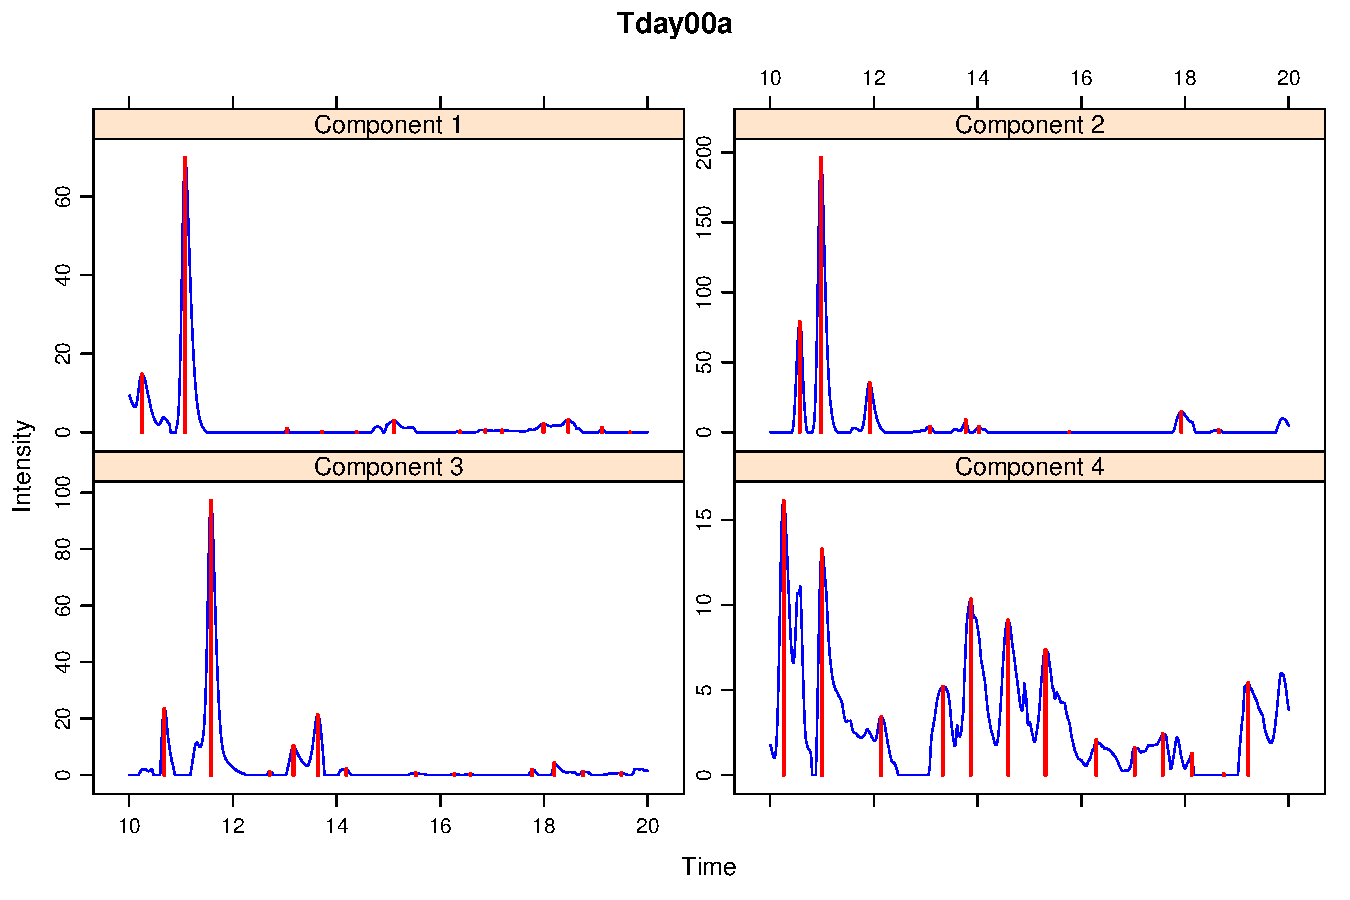
\includegraphics{stickPTW-003}
\caption{Some elution profiles from the first sample in the grape data set
  (blue continuous lines). Peaks, obtained after peak picking with a
  very simple algorithm, are indicated with red vertical lines.}
\label{fig:dadProfiles}
\end{figure}
Note that some less important peaks are missed, in particular peaks
near the edges of the retention time range, and shoulder peaks. 

The data are available in two objects, \code{grape.peaks} and
\code{grape.profiles}, both
nested lists, with the samples at the first level and the MCR
components at the second level. As the names suggest, the first
contains peaks (for each component a number of combinations of
retention time and intensity), and the second contains the elution
profiles for each of the components at all time points. As an example, 
the number of peaks in each sample/component combination can be assessed
by the following command:
\begin{Schunk}
\begin{Sinput}
> sapply(grape.peaks, function(x) sapply(x, nrow))[1:8, 1:7]
\end{Sinput}
\begin{Soutput}
     Tday00a Tday00b Tday01 Tday03 Tday04 Tday09 Tday10
[1,]      13      13     15     12     13     16     13
[2,]       9      10     10     10      7     10      6
[3,]      13      14     18     15     15     14     15
[4,]      13      13     13     13     13     15     14
[5,]      11      14     12     11     12     13     11
[6,]      15      16     16     15     14     16     14
[7,]       9      11      9      7      9     12      8
[8,]       6      11      8      6      8      8      8
\end{Soutput}
\end{Schunk}
where for reasons of space we restrict the output to the first eight
components and the first seven samples. Clearly, there is some 
difference in the number of peaks, not only for each component, but
also over time.

Closer inspection of the peaks in the MCR component over
the different samples reveals that there are some differences in
retention times. Component 2, for instance, has few peaks and
therefore is easy to inspect -- the next code shows the retention time
of the largest feature in this component across all samples:
\begin{Schunk}
\begin{Sinput}
> sapply(grape.peaks, function(x) {
+   big.idx <- which.max(x[[2]][,"I"])
+   as.numeric(rownames(x[[2]])[big.idx])
+ })
\end{Sinput}
\begin{Soutput}
Tday00a Tday00b  Tday01  Tday03  Tday04  Tday09  Tday10 
  10.98   10.80   10.94   10.91   10.94   10.99   10.94 
 Tday11  Tday13  Tday15  Tday17  Tday21  Tday24  Tday28 
  10.95   11.09   10.67   10.57   10.89   10.89   10.90 
\end{Soutput}
\end{Schunk}
Assuming that the biggest peak is actually
the same compound in all cases, we see a maximal retention time
difference of almost one minute.

Alignment of the profiles using the ptw function is easy, and works
pretty well. We choose (rather arbitrarily) the first injection as a
reference sample. This is usually not the best choice, since retention
time differences are likely to be biggest when comparing the extremes
of the sequence -- often, a sample from the middle is selected as a
reference. Since the retention time deviations here are caused by
environmental fluctuations in temperature rather than by a slower
process like column degradation, it is expected that the choice of a
reference here does not make much of a difference. We will create one
single warping function that optimizes the overlap in all fourteen MCR
components simultaneously, and use \code{system.time} to get an
impression on the speed of the warping. All parameters have been kept
to the system defaults; in particular, a quadratic warping function is
fitted.
\begin{Schunk}
\begin{Sinput}
> library(ptw)
> system.time(grape.profwarp <- 
+   lapply(grape.profiles[-1],
+          function(y) ptw(t(grape.profiles[[1]]), t(y), mode = "forward",
+                          warp.type = "global", trwdth = 40)))
\end{Sinput}
\begin{Soutput}
   user  system elapsed 
 11.763   0.032  11.795 
\end{Soutput}
\end{Schunk}

In comparison, the warping of the peak positions is much faster --
note that each profile contains 1,000 time points, whereas the maximal
number of peaks in one component is less than 20. So what exactly does
``much faster'' mean? We can find out by using function \code{stptw}
instead of \code{ptw}. Note that a few things change in the
call. We now use peak lists rather than lists of elution
profiles. In stick-based warping, the only possible warping type is
the \code{"global"} warping, so this argument is no longer
needed. Here goes: 
\begin{Schunk}
\begin{Sinput}
> system.time(grape.stickwarp <- 
+   lapply(grape.peaks[-1], 
+          function(y) 
+            stptw(grape.peaks[[1]], y, trwdth = 40)))
\end{Sinput}
\begin{Soutput}
   user  system elapsed 
  1.137   0.000   1.136 
\end{Soutput}
\end{Schunk}
That is a speed increase of almost an order of magnitude -- not bad!

How good is the agreement between the two types of warping? First of
all, we can look at the warped profiles, and the positions of the
warped peaks. The same components as seen in
Figure~\ref{fig:dadProfiles}, but now for the last sample in the
sequence, are shown in Figure~\ref{fig:warpedProfiles}.
\begin{figure}[tb]
  \centering
    \setkeys{Gin}{width=.95\textwidth}
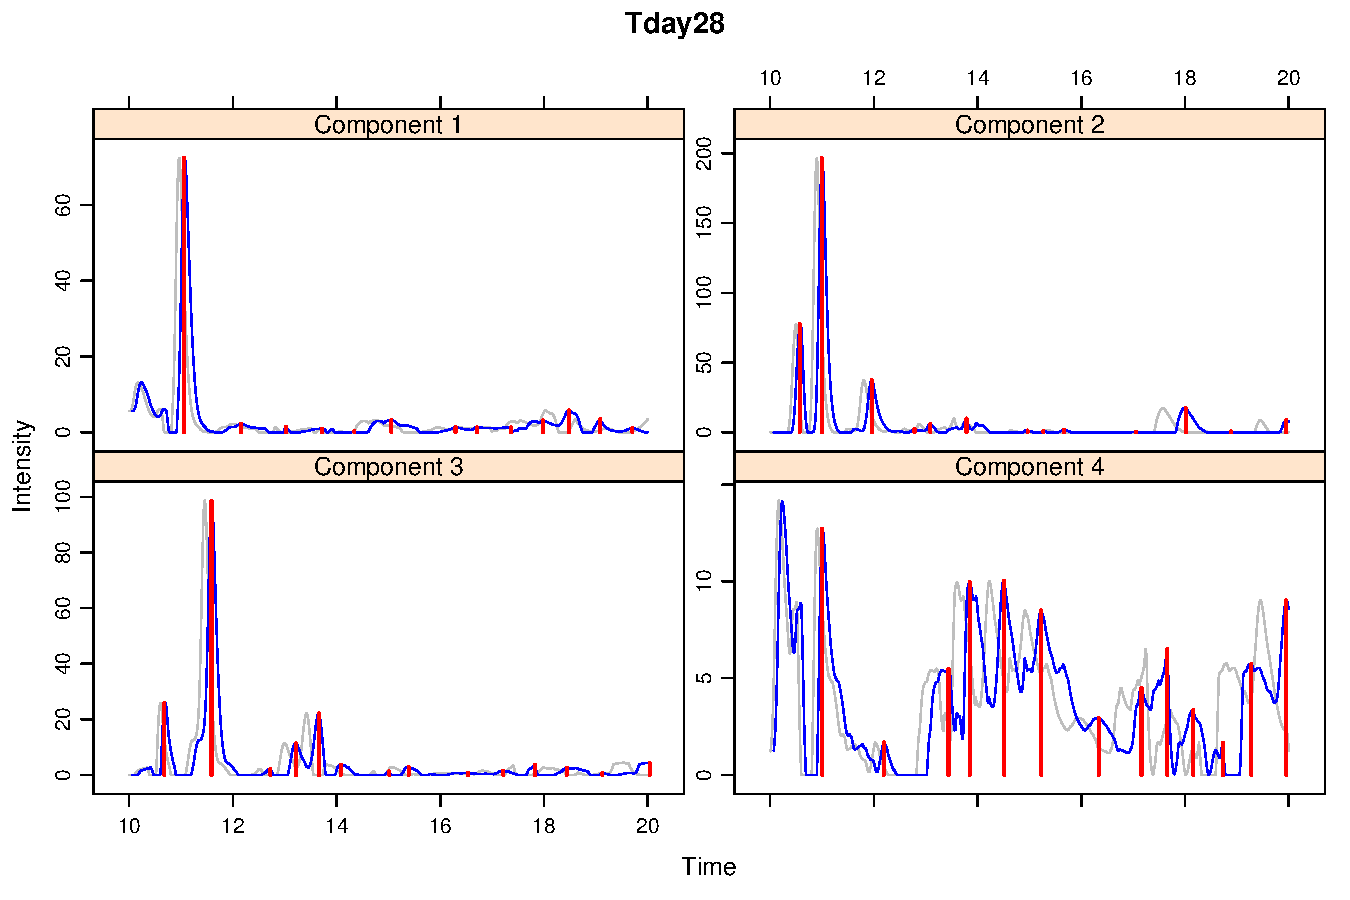
\includegraphics{stickPTW-009}
\caption{Warped elution profiles and peak positions from the last
  sample; the figure shows the same components as those in
  Figure~\protect\ref{fig:dadProfiles}. Profiles in gray show the
  original time profiles, those in blue the profiles after
  warping. Red vertical segments show sticks after warping.}
\label{fig:warpedProfiles}
\end{figure}
The agreement between the peaks in the blue warped profiles and the
warped peaks, shown in red, is excellent. There is one case, in
component 4, where a major peak is not picked because it is too close
to the boundary of the time window -- note that in the reference
sample, Tday00a, the peak \emph{is} found. This kind of errors can
easily be corrected by either more sophisticated peak picking
algorithms or simply taking a larger time window.

\begin{figure}[tb]
  \setkeys{Gin}{width=0.475\textwidth}
  \centering
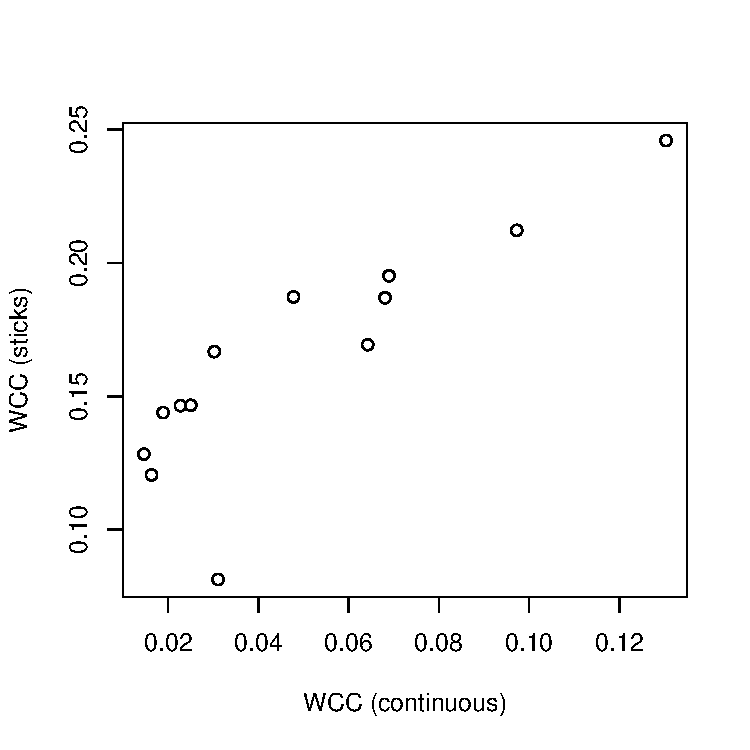
\includegraphics{stickPTW-010}
\caption{Comparison of WCC values from the continuous warping (x axis)
and stick warping (y axis) of the grape DAD data.}
\label{fig:wccComparison}
\end{figure}
Apart from the agreement between warped profiles and peak positions,
one can also inspect the warping objects to see if both warpings lead
to the same result. The values of the WCC quality criterion for
profile- and stick-based warpings are not directly comparable, even
though they both use the same triangle
width. Figure~\ref{fig:wccComparison} shows this. The reason is that
the data are different: in general the profile-based WCC values are
lower (indicating more agreement) because they take into account large
areas in which there is no or very little signal, which positively
contributes to the evaluation criterion.

Luckily, we can use one of the big advantages of parametric time
warping here, viz. the existance of an explicit warping function. This
means we can directly warp the continuous profiles using the warping
function obtained from the sticks. The result can then be compared
with the result of the warping of the continuous profiles. In
Figure~\ref{fig:warpComparison} this is done, with the warping
functions of the continuous data on the left, and those of the sticks
on the right. Clearly, both sets of warping functions are extremely similar.
\begin{figure}[bt]
  \centering
  \setkeys{Gin}{width=\textwidth}
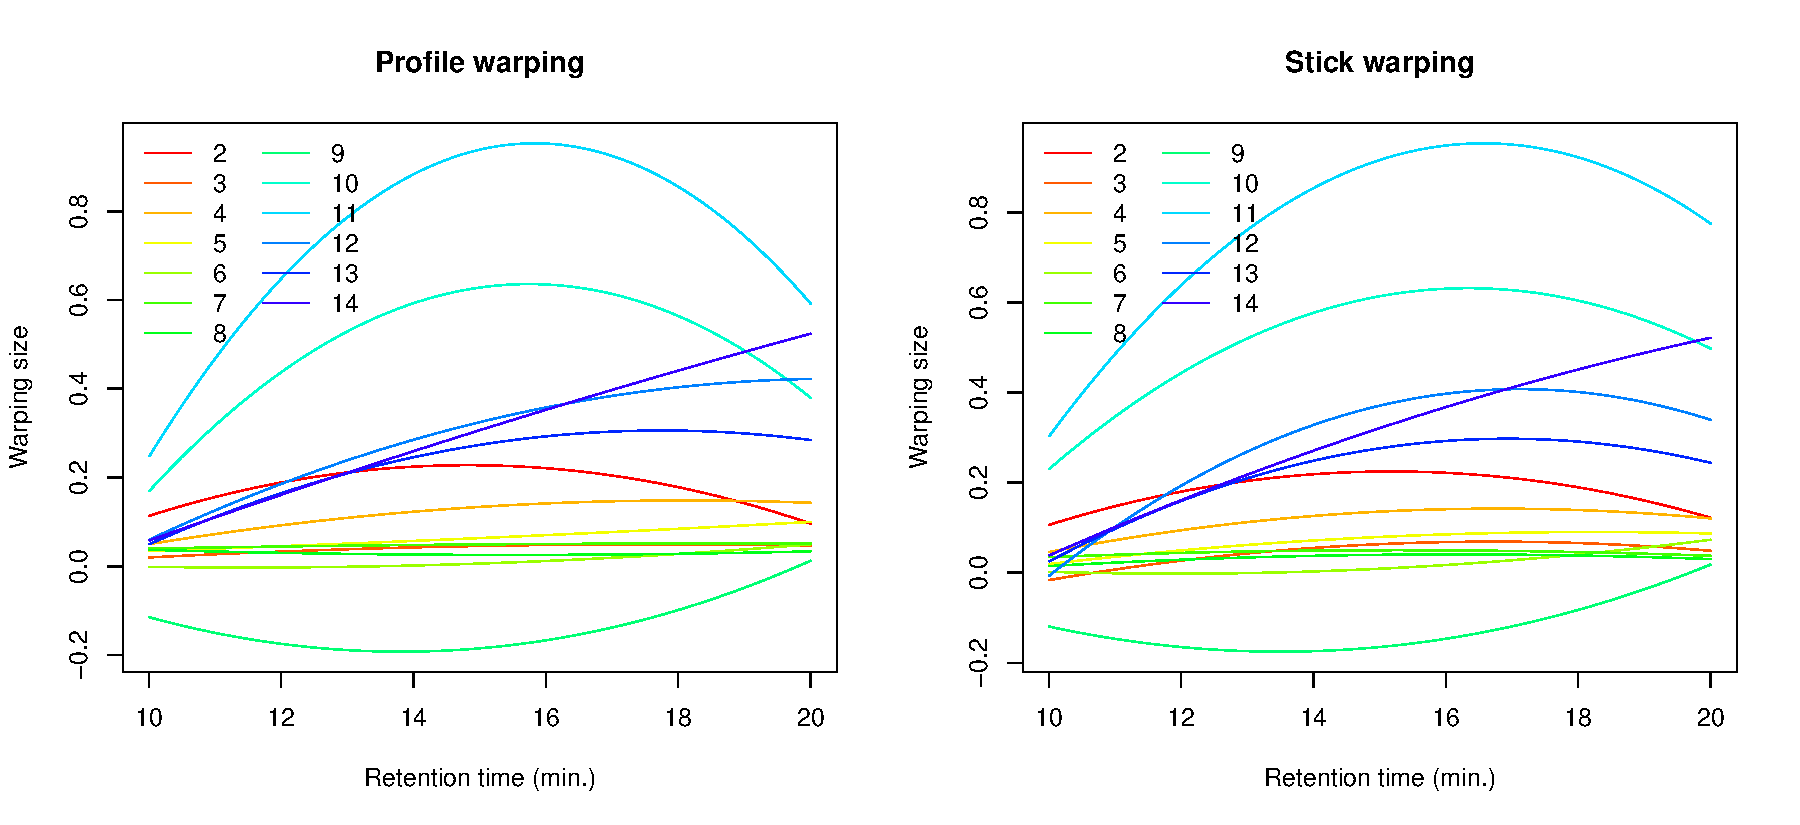
\includegraphics{stickPTW-011}
\caption{Grape DAD data: the 13 warping functions for continuous data
  (left) and sticks (right) -- the first of the 14 samples is taken as
  the reference. The $x$ axis presents the time, and the
  $y$ axis the size of the time correction, where a positive value
  indicates a shift to the right.}
\label{fig:warpComparison}
\end{figure}
We can warp the peaks with both sets of warping functions, and compare
the WCC values:
\begin{Schunk}
\begin{Sinput}
> ## warp peaks according to continuous warping functions
> grape.warped.peaks <- 
+   lapply(2:length(grape.peaks),
+          function(ii) 
+            lapply(grape.peaks[[ii]],
+                   function(x) {
+                     new.times <- warp.time(x[,"rt"],
+                                            t(grape.profwarp[[ii-1]]$warp.coef))
+                     x[,"rt"] <- new.times
+                     x}))
> ## calculate WCC values for each sample and each ALS component
> profWCCs <-
+   1-sapply(grape.warped.peaks,
+            function(x) 
+              mapply(wcc.st, x, pat2 = grape.peaks[[1]], trwidth = 40))
> ## and the result is:
> mean(profWCCs)
\end{Sinput}
\begin{Soutput}
[1] 0.1699119
\end{Soutput}
\begin{Sinput}
> ## compare that to the WCC value obtained in the stick warping:
> mean(sapply(grape.stickwarp, "[[", "crit.value"))
\end{Sinput}
\begin{Soutput}
[1] 0.1639269
\end{Soutput}
\end{Schunk}
They are virtually equal, indicating that warping the profiles gives
the same result as warping the peaks, the latter, of course, being
much faster.

\section{Analysis of LC-MS data from apples}
This section shows a more challenging application of peak-based
parametric time warping, coming from the field of untargeted
metabolomics. Typically, one sample leads to thousands of peaks, that
need to be aligned with the features found in other samples in order
to draw any conclusions. A peak is defined by three characteristics:
the retention time, the mass-to-charge ratio, and the intensity. All
three are subject to experimental error, but the error in retention
time is by far the largest and most important, in particular when
comparing data that have not been measured in the same batch.

To align peaks, we start by defining \emph{m/z} bins of a specific
width, and construct a peak list for each bin. The result is very
similar in structure to the ALS components seen with the DAD data,
only more extensive: one can easily define hundreds or even thousands
of bins. Choosing a high resolution leads to many bins, but there
will be many cases where bins are empty, or contain only very few
peaks. Putting all \emph{m/z} values in one bin corresponds to
something like aligning using the total ion current (TIC), something
that is not going to be easy~\citep{Bloemberg2010}. On the other hand,
having too few peaks in individual bins may make the alignment 
harder because no information is available for the optimization
routine, and one will have to strike a balance between these two effects.
Note that this binning process does not mean that mass resolution is lost:
individual peaks are merely grouped for the purpose of retention time
alignment.

The total-ion current (TIC)
chromatograms of these data are shown in Figure~\ref{fig:tics}. To
show the deviations in retention times more clearly, the TICs are
shown for each class of apples separately, in order of injection. Note
how different the peaks in the standard mixture (at the top of the
figure) are, compared to the apple data.
\begin{figure}[tb]
\centering
\setkeys{Gin}{width=.9\textwidth}
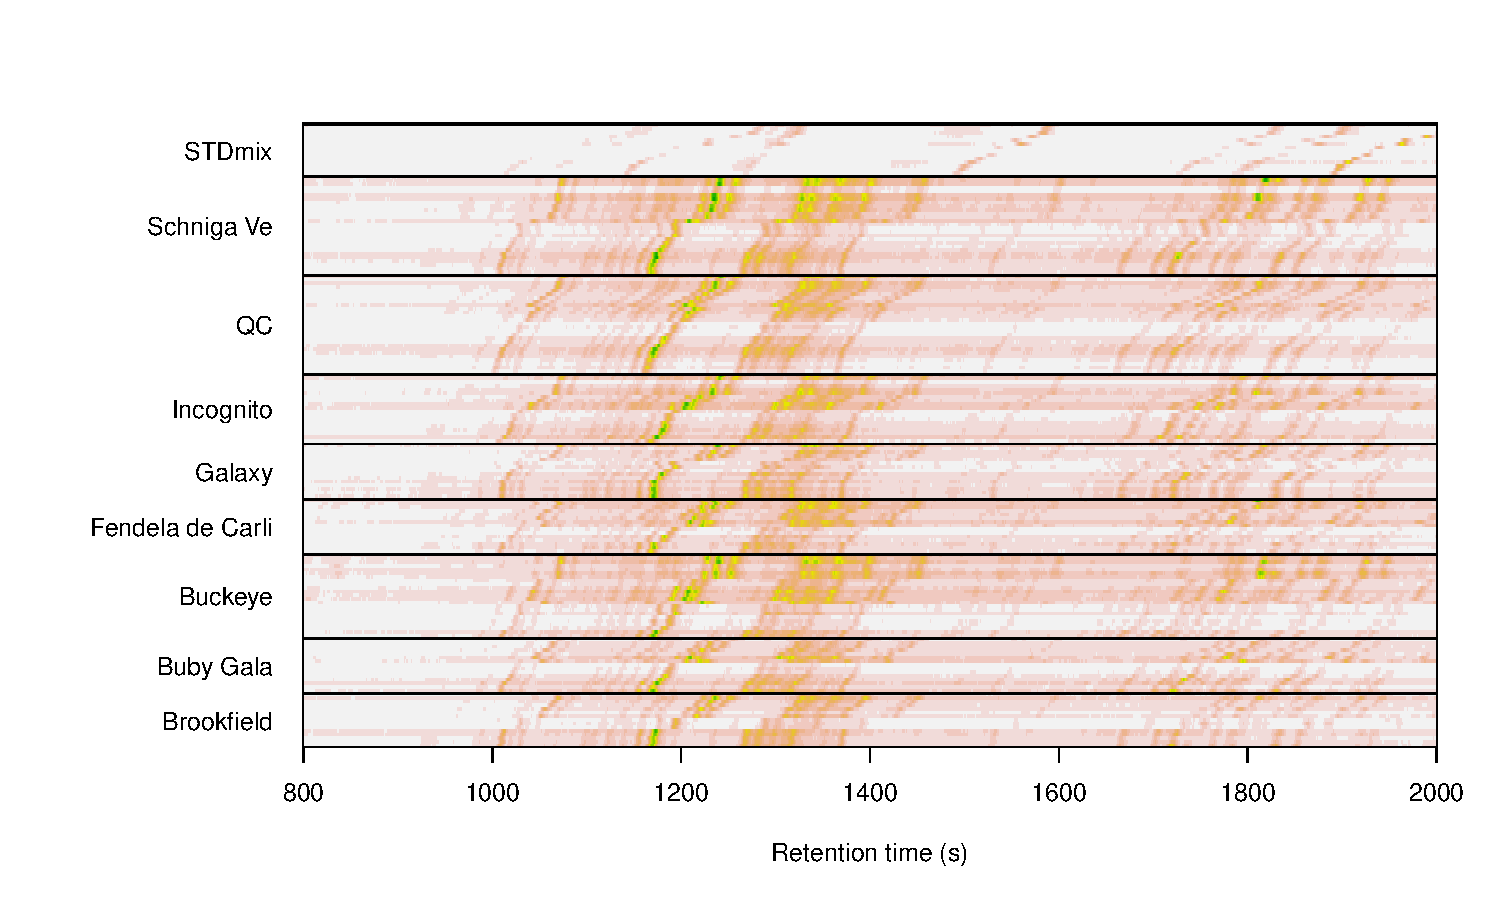
\includegraphics{stickPTW-013}
\caption{TICs of the LC-MS data -- intensities increase from white to
  brown to yellow to green. Injection
  classes are shown separately to show the gradual increase in
  retention times more clearly. The earliest injections are at the
  bottom of each class panel -- retention time shifts are up to one
  minute in size.}
\label{fig:tics}
\end{figure}

\subsection{Time warping of QC samples only}
For the apple data set, we start by considering only the 27 QC
samples. These have been measured at regular intervals,
covering the complete injection sequence. First we load the data, and
define bins of $1$ Dalton (i.e., very broad bins) in which peaks are
grouped. We only retain those bins containing peaks for at least half
the samples.
\begin{Schunk}
\begin{Sinput}
> QC.idx <- which(metaInf$Variety == "QC")
> QC.pks <- All.pks[QC.idx]
> QC.tics <- All.tics[QC.idx]
> ## divide the peak tables for all files into bins of size 1
> mzbins <- lapply(QC.pks, pktab2mzchannel, massDigits = 0)
> ## which bins occur in more than half of the files?
> allmasses <- 
+   table(unlist(lapply(mzbins, function(x) unique(names(x)))))
> mymasses <- as.numeric(names(allmasses[allmasses > 13]))
> length(mymasses)
\end{Sinput}
\begin{Soutput}
[1] 698
\end{Soutput}
\end{Schunk}
\begin{Schunk}
\begin{Sinput}
> ## now we can divide the peak tables again, focusing on these masses only 
> QC.mzlist <- lapply(QC.pks, pktab2mzchannel, 
+                     masses = mymasses, massDigits = 0)
\end{Sinput}
\end{Schunk}
The result is a nested list: for each of the 27 samples, 688
\emph{m/z} bins are considered in defining a warping
function. Clearly, this is much more challenging than the 14 DAD
samples with 14 components.

Let us define the first QC sample as the reference sample, and
calculate warping functions for all 26 other samples:
\begin{Schunk}
\begin{Sinput}
> QCwarpings <- 
+   lapply(2:length(QC.mzlist),
+          function(ii)
+            stptw(QC.mzlist[[1]], QC.mzlist[[ii]], trwdth = 50))
\end{Sinput}
\end{Schunk}
This step does take some time, so to prevent unnecessary waiting
during the development of this vignette, we cheat and save
intermediate results for later re-use.

We can visualize the effect of the warping by applying it to the
(continuous) total ion chromatogram (TIC) data, summarizing for
every time point the total amount of signal across all masses. Here,
we concentrate on the middle part of the chromatogram, between 800 and
2000 seconds:
\begin{Schunk}
\begin{Sinput}
> ## create a matrix of tic signals from the individual vectors of the
> ## samples - these are not measured at exactly the same times, so we
> ## use interpolation, one value for each second.
> QCticmat <- sapply(QC.tics, 
+                    function(x) 
+                      approx(x$scantime, x$tic, tictimes)$y)
> ## Now do the same, but apply the warping to the scantimes
> QCticmat2 <- 
+   sapply(seq(along = QC.tics),
+          function(ii) {
+            if (ii == 1) {
+              approx(QC.tics[[ii]]$scantime, 
+                     QC.tics[[ii]]$tic, 
+                     tictimes)$y
+            } else {
+              new.times <- warp.time(QC.tics[[ii]]$scantime, 
+                                     QCwarpings[[ii-1]]$warp.coef)
+              approx(new.times, QC.tics[[ii]]$tic, tictimes)$y
+            }})
\end{Sinput}
\end{Schunk}
\begin{figure}[tb]
  \centering
  \setkeys{Gin}{width=\textwidth}
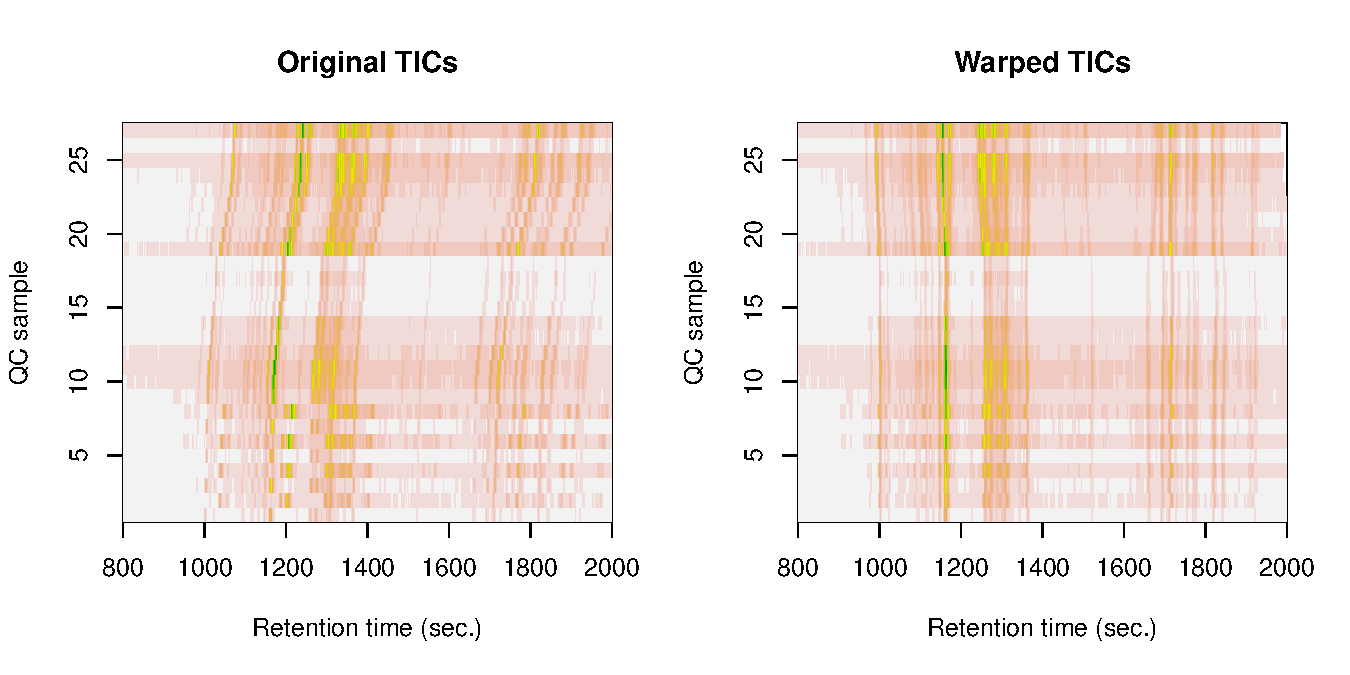
\includegraphics{stickPTW-019}
\caption{Original TICs of the apple QC samples (left), and TICS warped
  according to the warping functions from the peak lists
  (right). The injection order of the samples is from the bottom to
  the top.}
\label{fig:warpedQCTICs}
\end{figure}
The result is shown in Figure~\ref{fig:warpedQCTICs}. The left figure
clearly shows that peaks elute at later times in later QC samples,
whereas this trend is absent in the right figure, showing the
PTW-corrected TICs.

\subsection{Time warping of non-QC samples}
Defining the optimal warping works best if the majority of features is
present in all samples. Obviously, in real-life data sets this is very
often not the case, and the danger is that the optimization will end
up in a suboptimal solution. Two approaches can be used to remedy
this. The first assumes that subsequent injections are similar. That
is, in finding the optimal warping of sample $i+1$, one could start
from the result of warping sample $i$. Not only does this decrease the
result of false matches and an incorrect warping, it probably also
speeds up the procedure since fewer optimization steps are needed to
reach convergence.

However, this is not a fundamental solution to the fact that samples
may be very different, and that in such a case false matches between
peaks can be expected. The second possibility is to use the QC samples
mentioned earlier, and interpolate the warping functions of samples
injected between two QC samples. This again assumes a smooth shift in
retention times over the injection sequence, which usually is the case.
The retention times of the peaks in the apple samples can then be
warped according to the warping functions found in the QC warping,
through a simple process of linear interpolation between the QCs. We
can calculate warped retention times for the QC warpings and then
interpolate, or directly interpolate the warping coefficients:
\begin{Schunk}
\begin{Sinput}
> interpolate.warping <- function(rt, coef1, coef2, idx, 
+                                 type = c("coef", "time")) { 
+   weights <- abs(idx[2:3] - idx[1]) / diff(idx[2:3])
+   
+   type <- match.arg(type)
+   if (type == "time") {
+     rt1 <- warp.time(rt, coef1)
+     rt2 <- warp.time(rt, coef2)
+     crossprod(rbind(rt1, rt2), weights)
+   } else {
+     coefs <- crossprod(rbind(coef1, coef2), weights)
+     warp.time(rt, coefs[,1])
+   }
+ }
\end{Sinput}
\end{Schunk}

First we define the relevant QCs for each of the real samples:
\begin{Schunk}
\begin{Sinput}
> ## sort on injection order
> inj.order <- order(metaInf$InjectionNr)
> metaInf <- metaInf[inj.order,]
> All.pks <- All.pks[inj.order]
> All.tics <- All.tics[inj.order]
> ## pick out only the apple samples
> sample.idx <- which(!(metaInf$Variety %in% c("QC", "STDmix")))
> QC.idx <- which(metaInf$Variety == "QC")
> ## store the IDs of the QC samples around each sample
> neighbours.idx <- t(sapply(sample.idx,
+                            function(x) {
+                              c(x, 
+                                max(QC.idx[QC.idx < x]),
+                                min(QC.idx[QC.idx > x]))
+                            }))
> head(neighbours.idx, 9)
\end{Sinput}
\begin{Soutput}
      [,1] [,2] [,3]
 [1,]    7    5   14
 [2,]    8    5   14
 [3,]    9    5   14
 [4,]   10    5   14
 [5,]   11    5   14
 [6,]   12    5   14
 [7,]   13    5   14
 [8,]   15   14   21
 [9,]   16   14   21
\end{Soutput}
\end{Schunk}
So now we know what warpings to use for each of the sample. For
example, let's look at the fifth sample, injected at position 12. This
is flanked by the fourth and fifth QC samples, at positions 5 and 14:
\begin{Schunk}
\begin{Sinput}
> relevant.warpings <- which(QC.idx %in% c(5, 14)) - 1
> ## Original data:
> head(All.pks[[12]][,c("mz", "rt", "maxo", "sn")])
\end{Sinput}
\begin{Soutput}
           mz       rt      maxo        sn
[1,] 57.06821 1299.491  7.088608  7.150621
[2,] 60.07875 1368.869 12.151901 10.056416
[3,] 67.05031 1370.171  7.088608  5.346768
[4,] 69.06414 1686.200 14.177216  9.407192
[5,] 69.06279 1845.409 14.177216  6.286520
[6,] 69.06596 1616.806  9.113922  4.191239
\end{Soutput}
\begin{Sinput}
> ## the weighted average of the warpings of the 2 QC samples
> interpolate.warping(All.pks[[12]][1:6, "rt"],
+                     QCwarpings[[relevant.warpings[1]]]$warp.coef,
+                     QCwarpings[[relevant.warpings[2]]]$warp.coef,
+                     neighbours.idx[5,],
+                     type = "time")
\end{Sinput}
\begin{Soutput}
         [,1]
[1,] 1270.069
[2,] 1338.654
[3,] 1339.941
[4,] 1651.215
[5,] 1807.324
[6,] 1583.025
\end{Soutput}
\begin{Sinput}
> ## one warping, obtained by the weighted average of the warping coefs
> interpolate.warping(All.pks[[12]][1:6, "rt"],
+                     QCwarpings[[relevant.warpings[1]]]$warp.coef,
+                     QCwarpings[[relevant.warpings[2]]]$warp.coef,
+                     neighbours.idx[5,],
+                     type = "coef")               
\end{Sinput}
\begin{Soutput}
[1] 1270.069 1338.654 1339.941 1651.215 1807.324 1583.025
\end{Soutput}
\end{Schunk}
Clearly, the results of the two types of warping are the
same. Calculating average coefficients is more efficient, so that is
the default in our function. Now, let's do this for all the samples,
where we have to remember not only to correct the retention time but
also the intervals around the retention times:
\begin{Schunk}
\begin{Sinput}
> corrected.pks <- 
+   lapply(1:nrow(neighbours.idx),
+          function(pki) {
+            smp.idx <- which(names(All.pks) == 
+                                 metaInf[neighbours.idx[pki, 1], "file.name"])
+            QC1 <- which(QC.idx == neighbours.idx[pki, 2]) - 1
+            QC2 <- which(QC.idx == neighbours.idx[pki, 3]) - 1
+            
+            coef1 <- QCwarpings[[QC1]]$warp.coef
+            coef2 <- QCwarpings[[QC2]]$warp.coef
+            
+            cpk <- All.pks[[smp.idx]]
+            cpk[,"rt"] <- interpolate.warping(cpk[,"rt"],
+                                              coef1, coef2,
+                                              neighbours.idx[pki,])
+            cpk[,"rtmin"] <- interpolate.warping(cpk[,"rtmin"],
+                                                 coef1, coef2,
+                                                 neighbours.idx[pki,])
+            cpk[,"rtmax"] <- interpolate.warping(cpk[,"rtmax"],
+                                                 coef1, coef2,
+                                                 neighbours.idx[pki,])
+            cpk
+          })
> names(corrected.pks) <- metaInf[neighbours.idx[,1], "file.name"]
\end{Sinput}
\end{Schunk}
Applying the peak-based warpings to the TICs is done following exactly
the same line as earlier. First we correct all apple profiles:
\begin{Schunk}
\begin{Sinput}
> samp.tics <- All.tics[sample.idx] ## only real apple samples
> Corr.tics <- 
+   lapply(seq(along = samp.tics),
+          function(ii) { ## no warping for the first sample, the reference
+            if (ii == 1) {
+              samp.tics[[1]] 
+            } else {
+              QC1 <- which(QC.idx == neighbours.idx[ii, 2]) - 1
+              QC2 <- which(QC.idx == neighbours.idx[ii, 3]) - 1
+              
+              coef1 <- QCwarpings[[QC1]]$warp.coef
+              coef2 <- QCwarpings[[QC2]]$warp.coef
+ 
+              new.times <- interpolate.warping(samp.tics[[ii]]$scantime, 
+                                               coef1, coef2, 
+                                               neighbours.idx[ii,])
+              list(tic = samp.tics[[ii]]$tic, scantime = new.times)
+            }})
\end{Sinput}
\end{Schunk}
A part of the time axis of these corrected TICs is
shown in Figure~\ref{fig:ticsCorr}. This figure should be compared
with Figure~\ref{fig:tics} -- again, we can see that within each class
the retention time shift has been corrected very well. There still is
some variation, but the large effects of the leaking column have been
eliminated, and the remaining variation is probably small enough to be
tackled with the usual retention time correction methods present in
\code{XCMS}.
\begin{figure}[tb]
\centering
\setkeys{Gin}{width=.8\textwidth}
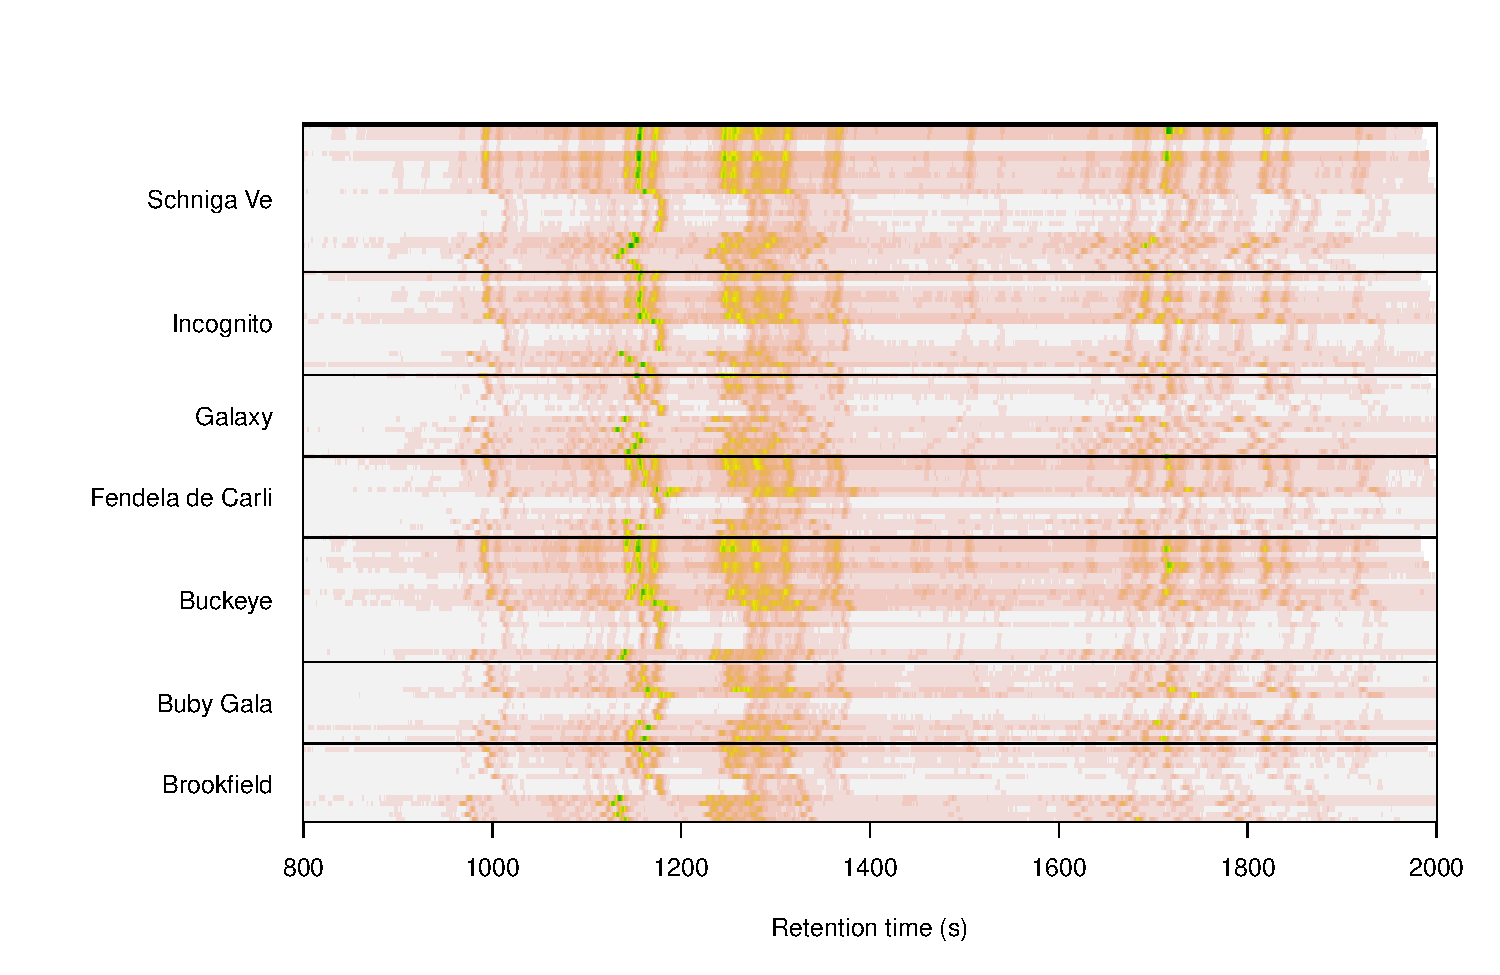
\includegraphics{stickPTW-025}
\caption{Corrected TICs of the LC-MS data, where the warping functions
  are obtained from the peak lists.}
\label{fig:ticsCorr}
\end{figure}

\section{Discussion}
Alignment can be a lengthy process, especially when many samples with
many time points need to be corrected. PTW has always been quite fast,
but the new peak-based form decreases computation times by an order of
magnitude or more, which significantly enhances its usefulness in
modern high-throughput applications. The new functionality could even
be used to fit higher-order warping functions with optimization
routines that are less likely to end up in local minima (but that need
more iterations) -- in some cases, we have seen that higher-order
warping coefficients can be quite variable, and this effect is
significantly reduced when using optimization methods like simulated
annealing or genetic algorithms. In practice, this functionality may
not be of crucial importance, but the possibility to investigate this
is an asset. In the \code{stptw} function experimental code has been
included, accessible through the argument \code{nGlobal}: this integer
indicates the number of global searches to be performed (using
function \code{nloptr} from the package with the same name, algorithm
``\code{NLOPT\_GN\_CRS2\_LM}'') prior to the normal steepest-descent
optimization. By default, \code{nGlobal = 0} when the polynomial
degree is three or smaller, and \code{nGlobal = 5} when higher-order
polynomials are used. Note that this takes quite a bit of computing time.

In this vignette we show that the peak-based warpings are very similar
to the original profile-based ones, and that forward and backward
warping modes can both be used for alignment of chromatographic
signals. We explicitly indicate how to use interpolated warpings,
based on QC samples, for aligning real samples, as already indicated
in \citet{Eilers2004}. This is a real bonus in cases where samples of
a quite different nature need to be warped: when comparing cases with
controls, for example, it may happen that large differences in
features lead a classical warping astray and that regular shift
corrections such as DTW or COW, that do not yield functional
descriptions of the optimal warpings, cannot be used.

We already mentioned the simple form of the PTW paradigm, requiring
the user only to choose a polynomial degree and the similarity
function. The latter choice is absent in the peak-based form of PTW,
which is only implemented for the WCC criterion (shown to outperform
the other criterion, Euclidean distance, in any case -- see
\citet{Bloemberg2010}). When analysing the peak lists in LC-MS data,
it will be necessary to aggregate the peaks into \emph{m/z}
bins\footnote{For nominal-mass GC data, this step is not even
  necessary.} of a certain width. This \emph{is} an extra step that
requires some attention from the user. Luckily, the choice of bin
width is not crucial. Wider bins lead to more peaks per bin and fewer
alignment steps, and are therefore faster; narrow bins contain few
peaks, but then there are more bins to process. In general, as long as
there are not too many empty bins, and there is not too much overlap
within individual bins, peak-based PTW will have no problems. In this
vignette, for example, we have not optimized the bin width at all.

\clearpage

\bibliographystyle{plainnat}
\bibliography{ptwbib} 

\clearpage
\section{Technical details}
\begin{Schunk}
\begin{Sinput}
> sessionInfo()
\end{Sinput}
\begin{Soutput}
R version 3.6.1 (2019-07-05)
Platform: x86_64-pc-linux-gnu (64-bit)
Running under: Ubuntu 18.04.3 LTS

Matrix products: default
BLAS:   /usr/lib/x86_64-linux-gnu/openblas/libblas.so.3
LAPACK: /usr/lib/x86_64-linux-gnu/libopenblasp-r0.2.20.so

locale:
 [1] LC_CTYPE=en_GB.UTF-8       LC_NUMERIC=C              
 [3] LC_TIME=nl_NL.UTF-8        LC_COLLATE=en_GB.UTF-8    
 [5] LC_MONETARY=nl_NL.UTF-8    LC_MESSAGES=en_GB.UTF-8   
 [7] LC_PAPER=nl_NL.UTF-8       LC_NAME=C                 
 [9] LC_ADDRESS=C               LC_TELEPHONE=C            
[11] LC_MEASUREMENT=nl_NL.UTF-8 LC_IDENTIFICATION=C       

attached base packages:
[1] stats4    parallel  stats     graphics  grDevices
[6] utils     datasets  methods   base     

other attached packages:
 [1] ptw_1.9-14          lattice_0.20-38    
 [3] metaMS_1.19.0       CAMERA_1.38.0      
 [5] xcms_3.4.0          MSnbase_2.8.0      
 [7] ProtGenerics_1.14.0 S4Vectors_0.20.1   
 [9] mzR_2.16.0          Rcpp_1.0.2         
[11] BiocParallel_1.16.0 Biobase_2.42.0     
[13] BiocGenerics_0.28.0

loaded via a namespace (and not attached):
 [1] vsn_3.50.0             splines_3.6.1         
 [3] foreach_1.4.4          Formula_1.2-3         
 [5] assertthat_0.2.0       BiocManager_1.30.4    
 [7] affy_1.60.0            latticeExtra_0.6-28   
 [9] RBGL_1.58.0            robustbase_0.93-3     
[11] impute_1.56.0          pillar_1.3.0          
[13] backports_1.1.2        glue_1.3.1            
[15] limma_3.38.2           digest_0.6.21         
[17] RColorBrewer_1.1-2     checkmate_1.8.5       
[19] colorspace_1.3-2       htmltools_0.3.6       
[21] preprocessCore_1.44.0  Matrix_1.2-15         
[23] plyr_1.8.4             MALDIquant_1.18       
[25] XML_3.98-1.16          pkgconfig_2.0.2       
[27] zlibbioc_1.28.0        purrr_0.3.3           
[29] scales_1.0.0           RANN_2.6              
[31] affyio_1.52.0          tibble_1.4.2          
[33] htmlTable_1.12         IRanges_2.16.0        
[35] ggplot2_3.1.0          nnet_7.3-12           
[37] lazyeval_0.2.1         MassSpecWavelet_1.48.0
[39] survival_2.43-1        magrittr_1.5          
[41] crayon_1.3.4           ncdf4_1.16            
[43] doParallel_1.0.14      MASS_7.3-51.1         
[45] foreign_0.8-71         graph_1.60.0          
[47] data.table_1.11.8      tools_3.6.1           
[49] stringr_1.3.1          munsell_0.5.0         
[51] cluster_2.0.7-1        bindrcpp_0.2.2        
[53] pcaMethods_1.74.0      compiler_3.6.1        
[55] mzID_1.20.0            rlang_0.4.0           
[57] nloptr_1.2.1           grid_3.6.1            
[59] rstudioapi_0.10        iterators_1.0.10      
[61] htmlwidgets_1.3        igraph_1.2.2          
[63] base64enc_0.1-3        gtable_0.2.0          
[65] codetools_0.2-16       multtest_2.38.0       
[67] R6_2.4.0               gridExtra_2.3         
[69] knitr_1.20             dplyr_0.7.8           
[71] bindr_0.1.1            Hmisc_4.1-1           
[73] stringi_1.2.4          rpart_4.1-15          
[75] acepack_1.4.1          DEoptimR_1.0-8        
[77] tidyselect_0.2.5      
\end{Soutput}
\end{Schunk}

\end{document}
